%\section{Making Counterexamples Actionable}
\label{sec:actionable}
We therefore desire AGREE counterexamples that are \textit{actionable}; that is, an explanation of the violation in terms that will quickly lead to a passing analysis (e.g., by making changes to the formal contract or model).
%
%In the following sections, we introduce AGREE-Dog, 
To achieve this, we implemented an interactive conversational copilot (AGREE-Dog) powered by GPT-4o and O3 multimodal generative AI models. It is specifically designed to assist AGREE users in identifying the root causes of counterexamples and applying targeted modifications during the model repair process, significantly reducing the turnaround time between verification attempts. The copilot is user-friendly and integrates seamlessly with the OSATE IDE (see Figure~\ref{fig:AGREEDOG}).

\begin{figure*}[t]
\centering
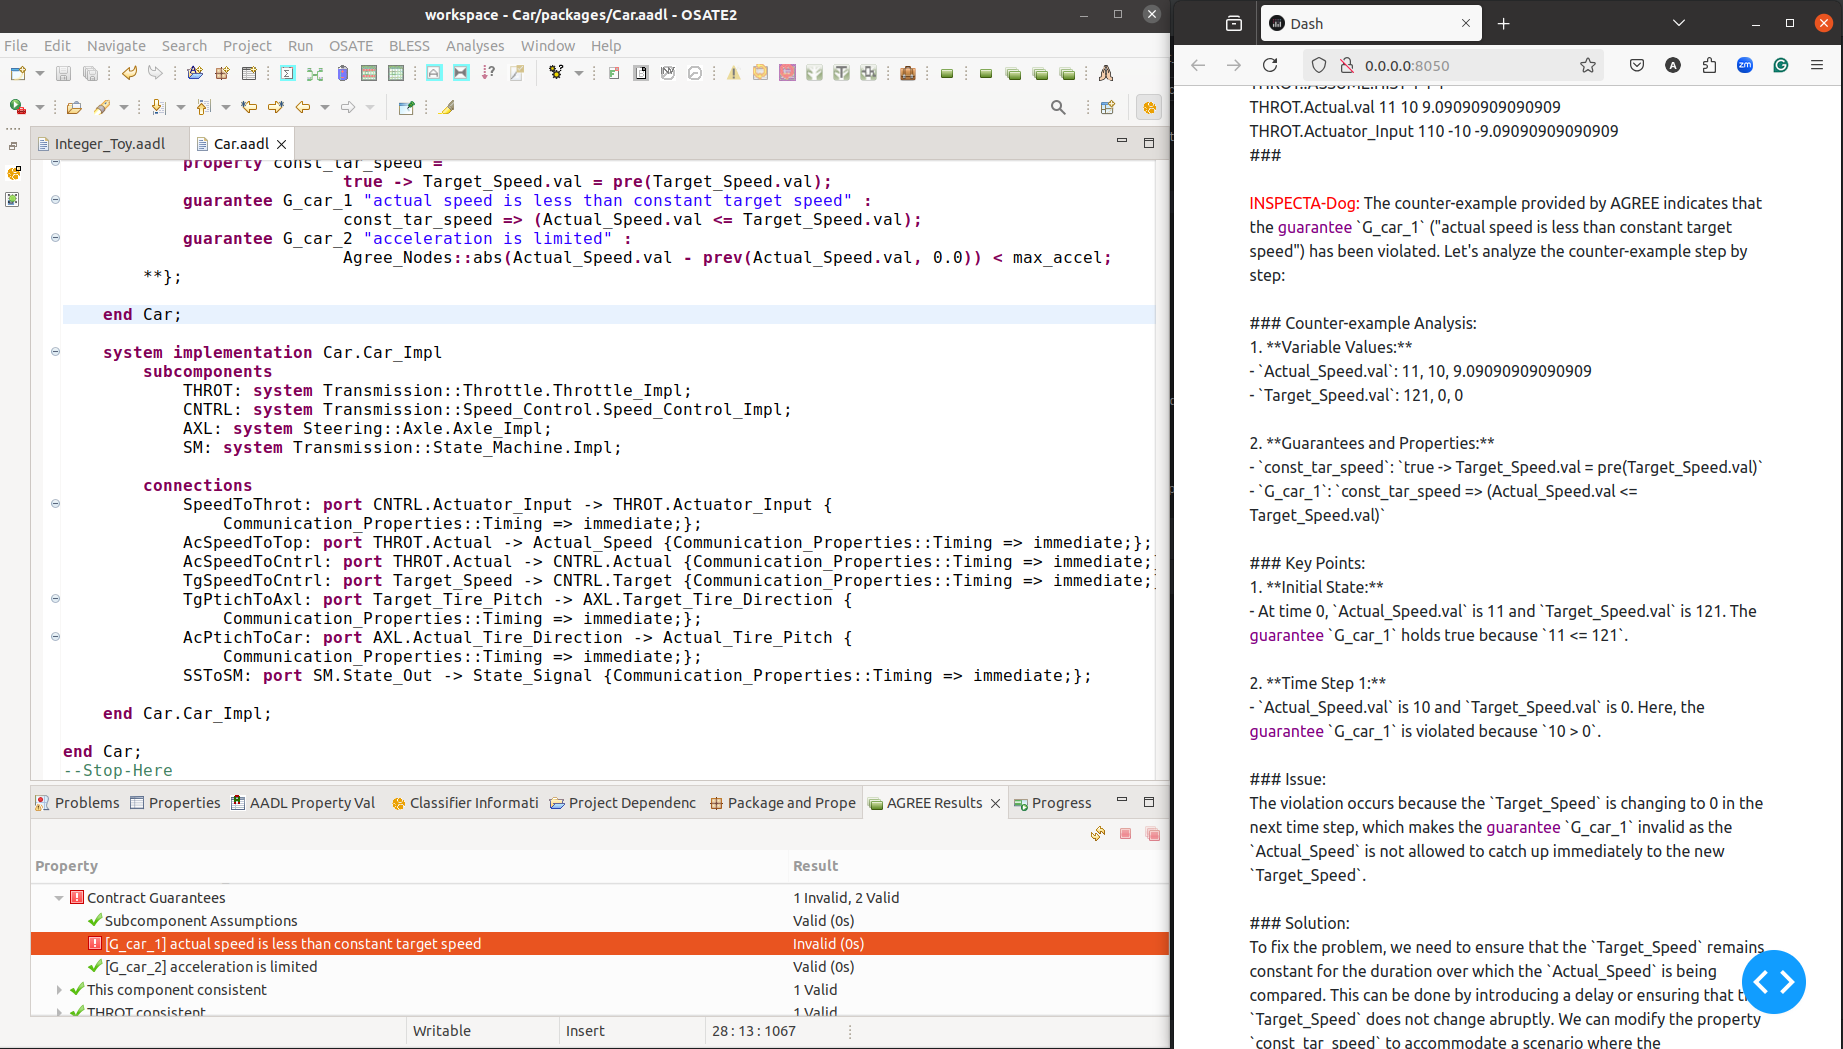
\includegraphics[height=0.6\textwidth, width=1.0\textwidth]{AGREE-DOG-high-rs.png}
\caption{AGREE-Dog copilot integrated within OSATE, providing an actionable explanation of a counterexample generated from the \texttt{Car} model.}
\label{fig:AGREEDOG}
\end{figure*}

In the remainder of this paper, we explore the motivations that drove the development of AGREE-Dog, describe its key architectural features, and evaluate its effectiveness within representative modeling and verification workflows.

